\documentclass[a4paper,12pt]{article}
\usepackage[a4paper,top=1.3cm,bottom=2cm,left=1.5cm,right=1.5cm,marginparwidth=0.75cm]{geometry}
\usepackage{cmap}
\usepackage{mathtext}
\usepackage[T2A]{fontenc}
\usepackage[utf8]{inputenc}
\usepackage[english,russian]{babel}
\usepackage{siunitx}
\usepackage{enumitem}
\usepackage{placeins}

\usepackage{graphicx}

\usepackage{wrapfig}
\usepackage{tabularx}
\usepackage{multirow}

\usepackage{hyperref}
\usepackage[rgb]{xcolor}
\hypersetup{
colorlinks=true,urlcolor=blue
}
\usepackage{amsmath,amsfonts,amssymb,amsthm,mathtools}
\usepackage{icomma}
\mathtoolsset{showonlyrefs=false}
\usepackage{euscript}
\usepackage{mathrsfs}
\DeclareMathOperator{\sgn}{\mathop{sgn}}
\newcommand*{\hm}[1]{#1\nobreak\discretionary{}
{\hbox{$\mathsurround=0pt #1$}}{}}

%%% Заголовок
\newcommand\labname{Геометрическая оптика}
\newcommand\labnumber{4.1.1}


\author{Макаров Лев Евгеньевич}
\title{Лабораторная работа №\labnumber

\labname
}

\date{\today}

\begin{document}
\begin{titlepage}
	\begin{center}
		{\large МОСКОВСКИЙ ФИЗИКО-ТЕХНИЧЕСКИЙ ИНСТИТУТ (НАЦИОНАЛЬНЫЙ ИССЛЕДОВАТЕЛЬСКИЙ УНИВЕРСИТЕТ)}
	\end{center}
	\begin{center}
		{\large Физтех-школа фотоники, электроники и молекулярной физики}
	\end{center}
	
	
	\vspace{4.5cm}
	{\huge
		\begin{center}
			{\bf Отчёт о выполнении лабораторной работы \labnumber}\\
			\labname
		\end{center}
	}
	\vspace{2cm}
	\begin{flushright}
		{\LARGE Автор:\\ Макаров Лев Евгеньевич \\
			\vspace{0.2cm}
			Б04-306}
	\end{flushright}
	\vspace{8cm}
	\begin{center}
		Долгопрудный 2025
	\end{center}
\end{titlepage}

\section{Введение}

\textbf{Цель работы:} 
\begin{enumerate}
	\item изучение свойств оптических систем: определение фокусных расстояний линз
    \item определение фокусных расстояний и положения главной и фокальной плоскостей сложной оптической системы
    \item изучение аббераций оптических систем.
\end{enumerate}

\textbf{В работе используются:} оптическая скамья с набором рейтеров, положительные и отрицательные линзы, экран, осветитель с ирисовой диафрагмой, зрительная труба, кольцевые диафргамы, линейка.


\section{Теоретические сведения}


\subsection*{Определения фокусных расстояний}
Формула тонкой линзы имеет вид
\begin{equation}
    \frac{1}{f} = \frac{1}{a} + \frac{1}{b},
\end{equation}
\noindent
где $f$ -- фокусное расстояние, $a$ -- расстояния от предмета до линзы, $b$ -- расстояние от изображения до линзы.

\noindent
Для измерения фокусного расстояния тонкой собирающей линзы может использоваться схема с рис. 1. и формула (2).
\begin{equation}
    f = \frac{L^2 - l^2}{4L}
\end{equation}

\begin{figure}[H]
    \centering
    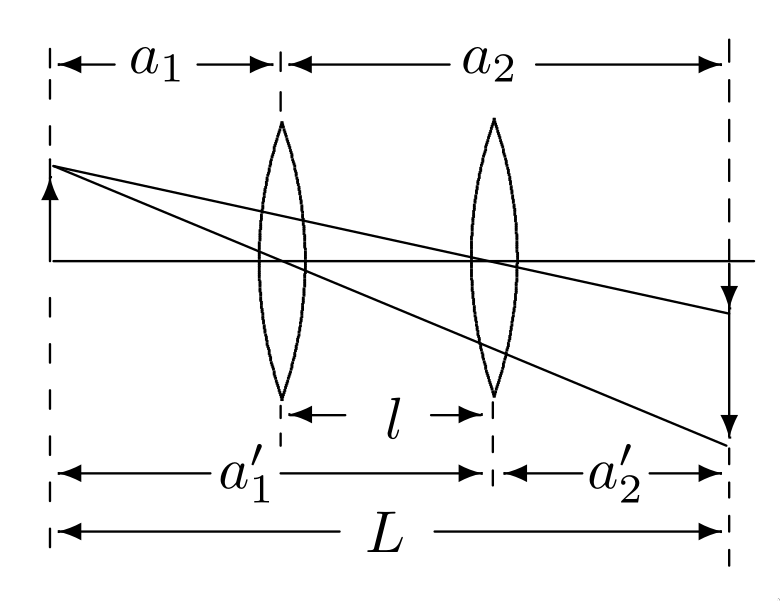
\includegraphics[scale=0.3]{pictures/plus_lense_focus.png}
    \caption{Схема измерения фокуса тонкой собирающей линзы}
\end{figure}

\noindent
Также фокусное расстояние тонкой собирабщей линзы можно измерить с помощью зрительной трубы, настроенной на бесконечность. Если расположить линзу между предметом и трубой и найти четкое изображение предмета, то расстояние от линзы до предмета будет равно фокусному.

\noindent
Для определения расстояние тонкой рассеивающей линзы поспользуемся схемой на рис. 2 и формулой тонкой линзы. Также можно восползоваться зриетльной трубой, настроенной на бесконечность. Если расположить предмет у нее в фокусе, то изображение переместиться в бесконечность, что можно проверить с помощью зрительной трубы.

\begin{figure}[H]
    \centering
    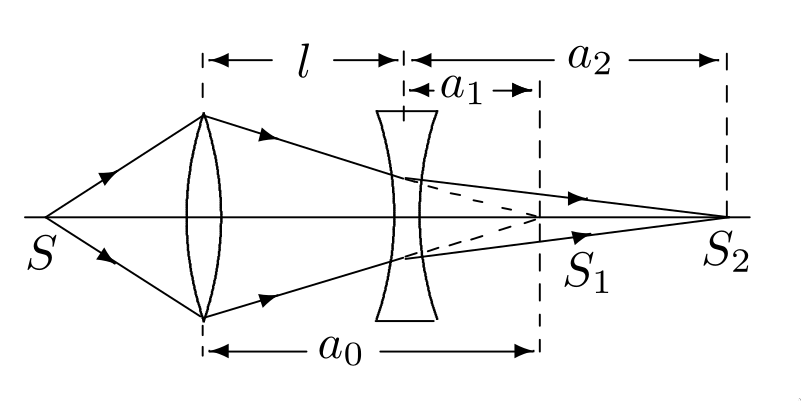
\includegraphics[scale=0.35]{pictures/neg_lense_focus.png}
    \caption{Схема измерения фокуса тонкой рассеивающей линзы}
\end{figure}

\noindent
Для определения фокусного расстояние и положения главных плоскостей сложной оптической системы может использоваться метод Аббе: схема на рис. 3 и формула (3).

\begin{figure}[H]
    \centering
    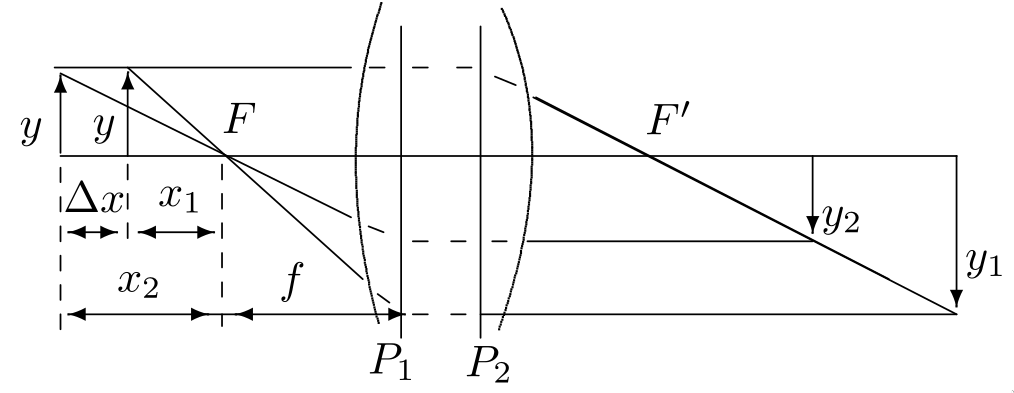
\includegraphics[scale=0.3]{pictures/system_focus.png}
    \caption{Схема определения фокусного расстояние и положения главных плоскостей сложной оптической}
\end{figure}

\begin{equation}
    f = \frac{\Delta x}{y / y_1 - y / y_2}    
\end{equation}

Пусть пучок света, попадающий в объектив, составляет с оптической осью угол $\varphi_1$, а пучок, выходящий из окуляра, — угол $\varphi_2$. Увеличение $\gamma$ зрительной трубы по определению равно
\begin{equation}
    \gamma = \frac{\tan \varphi_2}{\tan \varphi_1},
\end{equation}
но также из рис. 3 следует, что 
\begin{equation}
    \gamma_K = \frac{f_1}{f_2} = \frac{D_1}{D_2},
\end{equation}
где $D_1$ - ширина пучка, прошедшего через объектив, а $D_2$ - ширина пучка, вышедшего из окуляра

\subsection{Моделирование трубы Галилея}

\FloatBarrier
\begin{figure}[!ht]
    \centering
    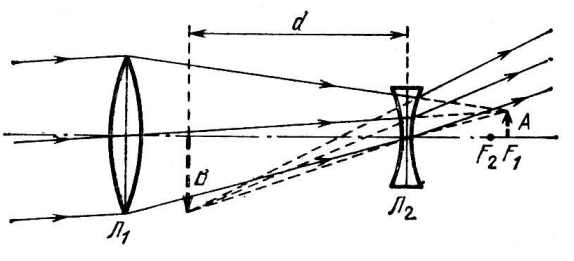
\includegraphics[width=9cm]{pictures/galileo_tube.png}
    \caption{Ход лучей в трубе Галилея}
    \label{fig:vac}
\end{figure}
\FloatBarrier

\subsection{Моделирование микроскопа}

\begin{figure}[h]
    \centering
    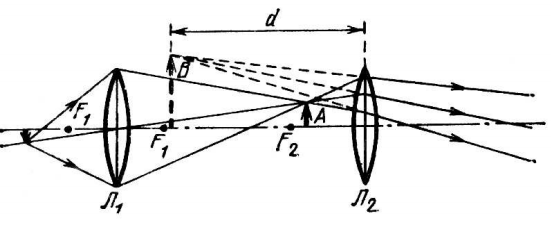
\includegraphics[width=9cm]{pictures/microscope_1.png}
    \caption{Ход лучей в микроскопе}
    \label{fig:vac}
\end{figure}


Ход лучей в микроскопе показан на рис. 6. Увеличение микроскопа вычисляется по формуле
    \begin{equation}
        \gamma_M = \Gamma_{o_b} \Gamma_{o_c} = \frac{\triangle}{f_1} \frac{L}{f_2},
    \end{equation}.
    
    \begin{figure}[h]
    \centering
    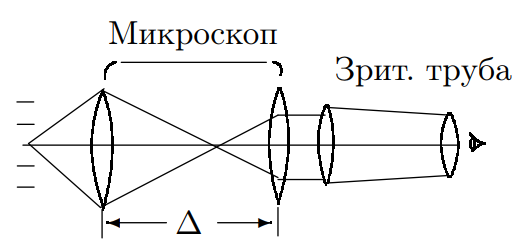
\includegraphics[width=9cm]{pictures/microscope_2.png}
    \caption{Схема микроскопа}
    \label{fig:vac}
\end{figure}   

\section{Результаты измерений и обработка данных}

\subsection*{0. Подготовка к работе}

\begin{enumerate}
    \item Определим какие линзы являются собирающими, а какие рассеивающими.
\end{enumerate}

\begin{itemize}
    \item собирающие: 3.1, 3.2, 3.3, 3.4, 3.6;
    \item рассеивающие: 3.5.
\end{itemize}

\begin{enumerate}[resume]
    \item Отцентрируем линзы относительно оптической оси, так чтобы свет источника проходил через центр всех линз.
\end{enumerate}


\subsection*{I. Определение фокусных расстояний линз с помощью подзорной трубы}

\begin{enumerate}
    \item Настроим подзорную трубу на бесконечность.
    \item Расположим одну из линз на оптической скамье на приблизительно фокусном расстоянии. Далее разместим за линзой подзорную трубу. Слегка перемещая линзу добьемся наиболее четкого изображения. Измерим фокусное расстояние линейкой.
    \item Перевернем линзу обратной стороной и измерим фокусное расстояние еще раз.
    \item Повторим измерения для остальных линз и результаты измерений запишем в таблицу \ref{table:1}.
\end{enumerate}


\begin{table}[!h]
	\caption{Фокусные расстояния всех линз}
	\label{table:1}	
	\begin{center}
		\begin{tabular}{|c|c|c|}
			\hline
			линза & $f$, см & $f_\text{обратное}$, см \\ \hline
			3.1	&	6.4 & 6.8 \\ \hline
			3.2	&	14.5 & 14.5 \\ \hline
			3.3	&	19.0 & 19.0 \\ \hline
			3.4	&	29.3 & 29.3 \\ \hline
			3.6	&	4.0 & 4.5 \\ \hline
		\end{tabular}
	\end{center}
\end{table}

\begin{enumerate}[resume]
    \item Повторим измерение для линзы 3.3 несколько раз и измерим среднеквадратичное отклонение $\sigma_f^\text{кв}$. Результаты измерений запишем в таблицу \ref{table:2}.
\end{enumerate}

\begin{table}[!h]
	\caption{Фокусные расстояния линзы 3.3}
	\label{table:2}	
	\begin{center}
		\begin{tabular}{|c|c|c|c|c|c|}
			\hline
			$f$, см & 19.0 & 18.9 & 19.0 & 18.8 & 19.2 \\ \hline
			$\sigma_f$, см & 0.5 & 0.5 & 0.5 & 0.5 & 0.5 \\ \hline
		\end{tabular}
	\end{center}
\end{table}


Тогда $\sigma_f^\text{кв} = 0.07$ см.

\begin{enumerate}[resume]
    \item Измерим фокусное расстояние отрицательной линзы. Разместим вспомогательную положительную линзу и получим на экране четкое изображение источника. Разместим отрицательную линзу между положительной и экраном. Уберем экран и разместим вместо него подзорную трубу. Перемещая отрицательную линзу получим четкое изображение предмета. Для повышения четкости вставим диафрагму. Измерим фокусное расстояние линзы как:
\end{enumerate}

\begin{equation*}
    f = l - a_0 = 27.2 - 35.8 \approx -8.6 \ \text{см}
\end{equation*}

\subsection*{II. Измерение фокусных расстояний линз по формуле тонкой линзы и методом Бесселя}

\begin{enumerate}
    \item Разместим одну из положительных линз на оптической скамье. Разместим экран на расстоянии $L = 91 \ \text{см} > 4f$ от предмета.
    \item Разместим исследуемую линзу между источником и экраном и получим на экране четкие изображения: одно увеличенное, а другое уменьшенное. Измерим соответствующие расстояния от источника до линзы $s_1$ и $s_2$.
\end{enumerate}

\begin{equation*}
    s_1 = 28.5 \ \text{см}; \ \ \ s_2 = 61.7 \ \text{см}
\end{equation*}
\begin{equation*}
    l = s_2 - s_1 = 33.2 \ \text{см}
\end{equation*}

\begin{enumerate}[resume]
    \item Вычислим фокусное расстояние двумя способами:
\end{enumerate}

Формула тонкой линзы:
\begin{equation*}
    f = \cfrac{1}{\frac{1}{s} + \frac{1}{L - s}}
\end{equation*}
\begin{equation*}
    f_1 = \cfrac{1}{\frac{1}{s_1} + \frac{1}{L - s_1}} = (19.6 \pm 0.4) \ \text{см}
\end{equation*}
\begin{equation*}
    f_2 = \cfrac{1}{\frac{1}{s_2} + \frac{1}{L - s_2}} = (19.9 \pm 0.2) \ \text{см}
\end{equation*}

Формула Бесселя:
\begin{equation*}
    f = \cfrac{L^2 - l^2}{4L} = (19.7 \pm 0.3) \ \text{см}
\end{equation*}

\begin{enumerate}[resume]
    \item Развернем линзу и повторим измерения
\end{enumerate}

\begin{equation*}
    f_1 = (19.5 \pm 0.4) \ \text{см}; \ \ \ f_2 = (19.9 \pm 0.2) \ \text{см}; \ \ \ f = (19.7 \pm 0.3) \ \text{см};
\end{equation*}


\subsection*{III. Измерение фокусных расстояний методом Аббе}

\begin{enumerate}
    \item Установим линзу между осветителем и экраном. Получим на экране четкое действительное изображение. Измерим линейное изображение предмета $y_0$ и предмета $y_1$.
    \item Отодвинем осветитель на расстояние $\Delta x = 5$ см от линзы. Передвинем экран к линзе на расстояние $\Delta x' = 57$ см, чтобы получилось четкое изображение. Измерим линейный размер изображения $y_2$.
    \item Рассчитаем фокусное расстояние методом Аббе:
\end{enumerate}

\begin{equation*}
    f = \cfrac{\Delta x'}{y_1/y_0 - y_2/y_0} = \cfrac{\Delta x}{y_0/y_2 - y_0/y_1}
\end{equation*}


\begin{table}[!h]
	\caption{Линейные размеры предмета и изображений}
	\label{table:3}	
	\begin{center}
		\begin{tabular}{|c|c|c|c|}
			\hline
			$y_0$, см & 2.1 & 1.4 & 0.6 \\ \hline
			$y_1$, см & 4.5 & 3.0 & 1.5 \\ \hline
            $y_2$, см & 9.0 & 6.3 & 3.1 \\ \hline
            $f$, см & 21.4 & 20.4 & 24.2 \\ \hline
            $f'$, см & 21.9 & 19.9 & 17.6 \\ \hline
		\end{tabular}
	\end{center}
\end{table}

\clearpage

\subsection*{IV. Сборка и изучение подзорной трубы Кеплера}

\begin{enumerate}
    \item В качестве коллиматора возьмем линзу 3.3, окуляра -- 3.1, объектива -- 3.4.
    \item С помощью подзорной трубы установим коллиматорную линзу перед источником, так чтобы он оказался в фокусе.
    \item Глядя в окуляр трубы, оценим количество ячеек, которое умещается в поле зрения. Угловой размер ячейки: $\alpha_0 = 1 / 4 = 0.25$.
    \item Объектив разместим сразу за коллиматором. Окуляр расположим на расстоянии $f_\text{об} + f_\text{ок}$ от объектива.
    \item При наблюдении глазом через окуляр телескопа наблюдаем увеличенное изображение сетки на поверхности источника. Повысим четкость, разместив диафрагму на коллиматоре.
    \item Измерим видимый размер изображения ячейки $\alpha = 1 / 2 = 0.5$.
\end{enumerate}

\begin{equation*}
    \gamma_\text{эксп} = \frac{\alpha}{\alpha_0} = 2
\end{equation*}
\begin{equation*}
    \gamma_\text{эксп} = \frac{f_\text{об}}{f_\text{ок}} = \frac{29.3}{6.8} \approx 4.3
\end{equation*}

Расхождении теории от эксперимента может быть из-за неточности измерений фокусных расстояний, неточности в сборке телескопа. Неточности в измерении угловых размеров.

\begin{enumerate}[resume]
    \item Измерим увеличение по диаметрам входного и выходного зрачков телескопа. $D_\text{об}$ -- диаметр светового пятна, падающего на объектив, $D_\text{ок}$ -- диаметр светового пятна за окуляром.
\end{enumerate}

\begin{equation*}
    \gamma = \frac{D_\text{об}}{D_\text{ок}} = \frac{1.9}{1} = 1.9
\end{equation*}


\subsection*{V. Сборка и изучение модели микроскопа}

\begin{enumerate}
    \item В качестве объектива используем линзу 3.6, а окуляра -- 3.1.
\end{enumerate}

\begin{equation*}
    \Delta = 4.5 \ \text{см}; 
\end{equation*}

\begin{equation*}
    \gamma_\text{экр} = \frac{L - f_\text{ок}}{f_\text{ок}} \cdot \frac{\Delta}{f_\text{об}} \approx 
\end{equation*}

\begin{enumerate}[resume]
    \item Разместим линзы согласно рассчетам. Источник разместим вблизи фокуса объектива. Глядя в окуляр и немного смещая предмет, добъемся четкого изображения сетки. Повысим четкость надев диафрагму на объектив.
    \item Для измерения увеличения установим за микроскопом экран. Слегка смещая предмет, добъемся четкого изображения на экране. Измерим его линейный размер. Рассчитаем линейное увеличение:
\end{enumerate}

\begin{equation*}
    \gamma = \frac{y_1}{y_0} = \frac{1.8}{1.4} \approx 1.3
\end{equation*}

\clearpage

\subsection*{VI. Изучение составной оптической системы}

\begin{enumerate}
    \item Используем линзы 3.5 и 3.6. Разместим их подставками плотно друг к другу и измерим расстояние между ними $l = 3.5$ см. Оценим фокусное расстояние:
\end{enumerate}

\begin{equation*}
    \frac{1}{f} = \frac{1}{f_1} + \frac{1}{f_2} + \frac{l}{f_1 f_2}
\end{equation*}

\begin{equation*}
    f = 4 \ \text{см}
\end{equation*}

\section{Вывод}

Были исследованы различные способы нахождения фокусных расстояний линзы. Наиболее эффективным оказался метод с использованием подзорной трубы -- все значения совпали в пределах погрешности. Также неплохо показал себя метод Бесселя. Метод Аббе не получился из-за ошибки в выполнении.

Также были собраны телескоп Кеплера и микроскоп и измерены их увеличения.





\end{document}